\section{Conclusion}\label{sec:conclusion}


We present our final models for the Franke function and the Grand Canyon terrain. 


\subsection{Franke function}
 
After performing the OLS analysis on the Franke function, it quickly became clear that a two-dimensional polynomial of order $d=5$ was the best model, i.e. yielding the lowest MSE. This can be seen most clearly from \Fig{model_complexity_ols} and \Fig{bias_variance_ols} we compare model of both higher and lower polynomial degree. A rough by-eye estimate of the MSE in these two cases is $\mathrm{MSE}\approx 0.16$ for the test data. This is confirmed in \Fig{cross-validation_ols} and \Fig{mse_hist_ols}, where the former yields a slightly higher MSE value. 

For the Ridge analysis we just assume that the polynomial degree found for OLS will yield the best result, and seek to find the optimal $\lambda$ only. One could argue that this is naive, so we should perhaps have allowed for the polynomial degree to change when performing Ridge analysis. However, with $d^\text{OLS}=5$, the optimal penalty parameter is found to be $\lambda^\mathrm{Ridge} = 7.85\cdot10^{-5}$ given to two significant figures. We have from \Fig{bootstrapping_ridge} and \Fig{mse_hist_ridge} that an approximate value of the MSE found for this model is $\mathrm{MSE} \approx 0.14$ for the test data. 

For the Lasso analysis we try to find a new optimal polynomial degree, which result in the maximum value of our grid $d=14$, which is not necessarily a bad model for a $N=20$ grid, since the penalty parameter drives unimportant features to zero. However, according to \Fig{cross-validation_lasso} and \Fig{bias_variance_lasso} there seems to be an optimal $\lambda\in[10^{-5}, 10^{-4}]$. However, the MSE value of $\approx 0.15$ of the same order for both OLS and Ridge. 

One could argue that Ridge yields a slightly lower MSE than OLS. However, these values are highly dependant on the method by which they were found, and the $k$-number in both bootstrap and cross-validation. The only sensible conclusion is thus that they yield approximately the same result. While OLS is less computationally expensive, and gives a simpler model altogether we further conclude that OLS with a polynomial degree $d^\text{OLS}=5$ is the model that fits the data best. 

We check this and plot the prediction model alongside the scaled data points. This can be seen in \Fig{franke_final_model} and the model is indeed good. 

\begin{figure}
    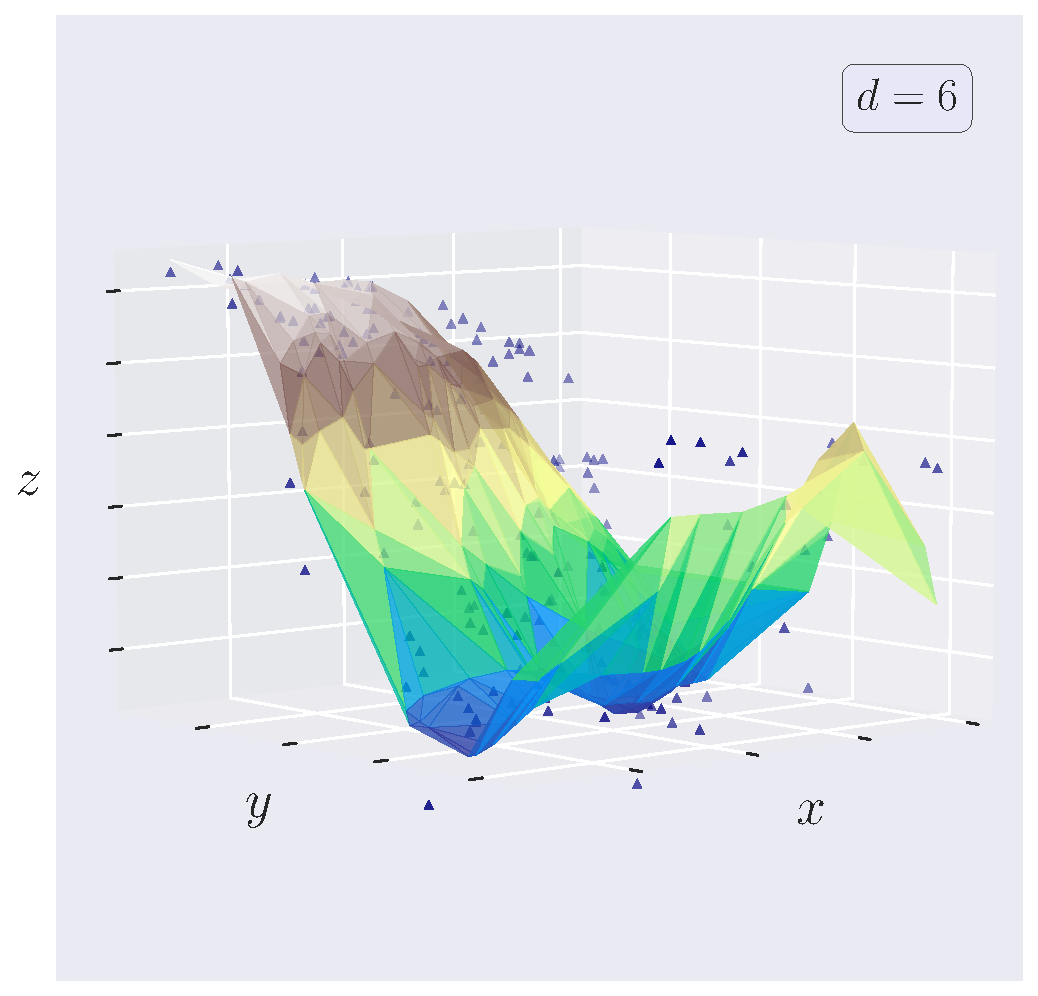
\includegraphics[width=\linewidth]{Franke/comparison3D_ols.pdf}
    \caption{Best fit model of the Franke function. The triangular points are the scaled data points, whilst the surface represent the corresponding prediction we get from an OLS estimate with $d=5$. }
    \label{fig:franke_final_model}
\end{figure}



\subsection{Grand Canyon terrain}

We got two models that in terms of MSE were almost equally good. The OLS model has $d^\text{OLS}=6$ and the Ridge model has $d^\text{Ridge}=18$ and $\lambda^\text{Ridge}=1.23\cdot10^{-4}$. The analysis yielded very similar prediciton errors for the two, see \Fig{gc_model_complexity_ols} and \Fig{gc_model_complexity_ridge}. However, as introduced in \Sec{Ridge}, the variance of the $\beta_j$'s are generally lower for the Ridge scheme than for the OLS scheme, and this is why we choose the former. The resulting terrain prediction is shown in \Fig{gc_final_model}.


\begin{figure}
    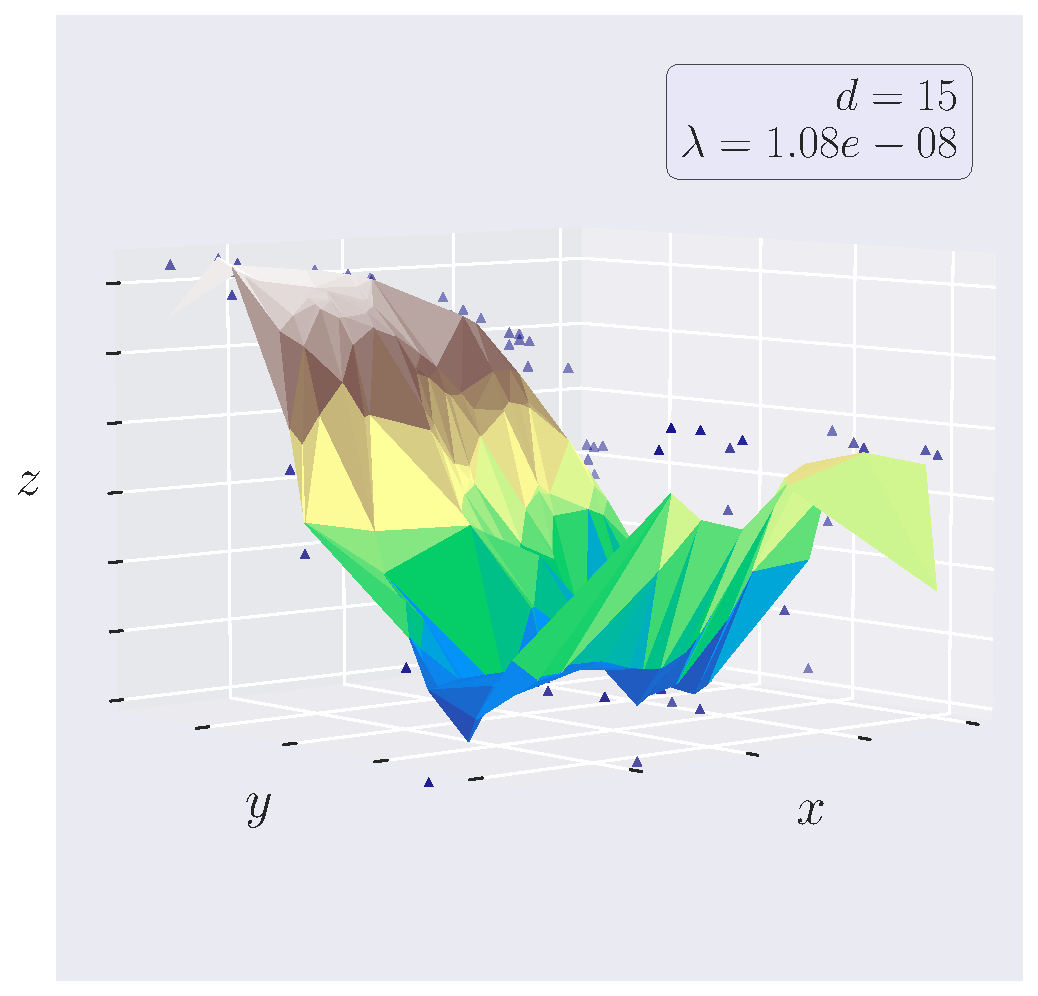
\includegraphics[width=\linewidth]{terrain/comparison3D_ridge.pdf}
    \caption{Best fit model of the terrain data. The triangular points are the scaled test data points, whilst the surface represents the corresponding prediction we get from a Ridge estimation with $d^\text{Ridge}=18$ and $\lambda^\text{Ridge}=1.23\cdot 10^{-4}$.}
    \label{fig:gc_final_model}
\end{figure}

The terrain is definitely recognisable to the Grand Canyon (\Fig{gc_data}, mind the angle). There is a tendency to flatten out by the edges as opposed to continuing downwards, which was the typical case with the OLS-models.
